\documentclass[letterpaper]{article} % DO NOT CHANGE THIS
\usepackage{aaai23}  % DO NOT CHANGE THIS
\usepackage{times}  % DO NOT CHANGE THIS
\usepackage{helvet}  % DO NOT CHANGE THIS
\usepackage{courier}  % DO NOT CHANGE THIS
\usepackage[hyphens]{url}  % DO NOT CHANGE THIS
\usepackage{graphicx} % DO NOT CHANGE THIS
\urlstyle{rm} % DO NOT CHANGE THIS
\def\UrlFont{\rm}  % DO NOT CHANGE THIS
\usepackage{natbib}  % DO NOT CHANGE THIS AND DO NOT ADD ANY OPTIONS TO IT
\usepackage{caption} % DO NOT CHANGE THIS AND DO NOT ADD ANY OPTIONS TO IT
\frenchspacing  % DO NOT CHANGE THIS
\setlength{\pdfpagewidth}{8.5in}  % DO NOT CHANGE THIS
\setlength{\pdfpageheight}{11in}  % DO NOT CHANGE THIS
\usepackage{algorithm}
\usepackage[noend]{algpseudocode}
\usepackage{amsmath}
\usepackage{amsthm}
\usepackage{amssymb,amsfonts}
\usepackage{xspace}
\usepackage{enumitem}
\usepackage{multicol}
\usepackage{multirow}
\usepackage{url}
\usepackage{soul}

\usepackage{nicematrix}
\usepackage{tikz}

\newtheorem{theorem}{Theorem}


\newtheorem{prop}{Proposition}
\newtheorem{condition}{Condition}

\newtheorem{remark}{Remark}
\newtheorem{definition}{Definition}
\newtheorem{claim}{Claim}
\newtheorem*{lemma*}{Lemma}
\newtheorem*{theorem*}{Theorem}
\newtheorem{example}{Example}
\newtheorem{lemma}{Lemma}

\newcommand{\lovasz}{{Lov\'asz}\xspace}
\newcommand{\nls}{\textsc{Nelson}\xspace}

\newcommand{\vect}[1]{\boldsymbol{\rm #1}}
\newcommand{\var}{\mathtt{var}}
\newcommand{\p}{\mathbb{P}}
\newcommand{\e}{\mathbb{E}}
\newcommand{\false}{\texttt{False}\xspace}
\newcommand{\true}{\texttt{True}\xspace}
\usepackage{newfloat}
\usepackage{listings}
\DeclareCaptionStyle{ruled}{labelfont=normalfont,labelsep=colon,strut=off} % DO NOT CHANGE THIS
\lstset{%
basicstyle={\footnotesize\ttfamily},% footnotesize acceptable for monospace
numbers=left,numberstyle=\footnotesize,xleftmargin=2em,% show line numbers, remove this entire line if you don't want the numbers.
aboveskip=0pt,belowskip=0pt,%
showstringspaces=false,tabsize=2,breaklines=true}
\floatstyle{ruled}
\newfloat{listing}{tb}{lst}{}
\floatname{listing}{Listing}


\setcounter{secnumdepth}{0} %May be changed to 1 or 2 if section numbers are desired.



\title{Learning Markov Random Fields for Combinatorial Structures via \\
Sampling through \lovasz Local Lemma}
\author{
Nan Jiang\equalcontrib\textsuperscript{\rm 1},
Yi Gu\equalcontrib\textsuperscript{\rm 2},
Yexiang Xue\textsuperscript{\rm 1}
}
\affiliations{
\textsuperscript{\rm 1} Department of Computer Science, Purdue University, USA\\
\textsuperscript{\rm 2} Department of Mathematics, Northwestern University, USA \\
\{jiang631, yexiang\}@purdue.edu, Yi.Gu@u.northwestern.edu
}



\begin{document}

\maketitle


\begin{abstract}

Learning to generate complex combinatorial structures satisfying constraints will have transformative impacts in many application domains.
However, it is beyond the capabilities of existing approaches due to the highly intractable nature of the embedded probabilistic inference.
Prior works spend most of the training time learning to separate valid from invalid structures but do not learn the inductive biases of valid structures.
We develop   \underline{NE}ural \underline{L}ov\'asz \underline{S}ampler (\nls), which embeds the sampler through \lovasz Local Lemma (LLL) as a fully differentiable neural network layer.
Our \nls-CD embeds this sampler
into the contrastive divergence learning process of Markov random fields.
\nls allows us to obtain valid samples from the current model distribution.
Contrastive divergence is then applied to separate these samples from those in the training set.
\nls is implemented as a fully differentiable neural net, taking advantage of the parallelism of GPUs.
Experimental results on several real-world domains reveal that \nls learns to generate 100\% valid structures, while baselines either time out or cannot ensure validity.
\nls also outperforms other approaches in running time, log-likelihood, and MAP scores.
\end{abstract}
\section{Introduction}
In recent years, tremendous progress has been made in generative modeling~\cite{DBLP:journals/neco/Hinton02,Tsochantaridis2005StructualSVM,goodfellow2014generative,kingma2013auto,Germain2015MADEMA,Larochelle2011Autoregressive,Oord2016PixelRN,arjovsky17WGAN,song2019generative,song21scoredifussion,murphy1999loopy,yedidia2001generalized,wainwright2006relaxation}.

Learning a generative model involves increasing the divergence in  likelihood scores  between the structures in the training set and those structures sampled from the current generative model distribution.
While current approaches have achieved successes in \textit{un-structured} domains such as vision or speech, their performance is degraded in the structured domain, because it is already computationally intractable to search for a valid  structure in a combinatorial space subject to constraints, not to mention sampling, which has a higher complexity.
In fact, when applied in a constrained domain, existing approaches spend most of their training time manipulating the likelihood of invalid structures, but not learning the difference between valid structures inside and outside of the training set.
In the meantime, tremendous progress has been made in automated reasoning \cite{Braunstein2005SurveyPA,AnHaHoTi2007,chavira2006compiling,VanHentenryck1989,GOGATE2012AndOr,Sang2005}. % for probabilistic inference over combinatorial structures.
Nevertheless, reasoning and learning have been growing independently for a long time. Only recently do ideas  emerge exploring the role of reasoning in learning~\cite{kusner17GrammarVAE,Jin2018JunctionTV,Dai2018SyntaxDirectedVA,Hu17ControlledTextGen,lowd2008learning,DBLP:conf/icml/DingMXX21}.



The \lovasz Local Lemma (LLL)~\cite{erdHos1973problems} is a classic gem in combinatorics, which at a high level, states that there exists a positive probability that none of a series of \textit{bad} events occur, as long as these events are \textit{mostly} independent from one another and are not too likely individually.
Recently, \citet{DBLP:journals/jacm/MoserT10} came up with an algorithm, which samples from the probability distribution proven to exist by LLL.
\citet{DBLP:journals/jacm/GuoJL19} proved that the algorithmic-LLL is an unbiased sampler %for the distribution %defined on valid instances
if those bad events satisfy the so-called ``extreme'' condition.
The expected running time of the sampler is also shown to be polynomial.
As one contribution of this paper, we offer proofs of the two aforementioned results using precise mathematical notations, clarifying a few descriptions not precisely defined in the original proof.
While this line of research clearly demonstrates the potential of LLL in generative learning (generating samples that satisfy all hard constraints), it is not clear how to embed LLL-based samplers into learning and no empirical studies have been performed to evaluate LLL-based samplers in machine learning.



In this paper, we develop   \underline{NE}ural \underline{L}ov\'asz \underline{S}ampler (\nls), which implements the LLL-based sampler as a fully differentiable neural network.
Our \nls-CD embeds \nls
into the contrastive divergence learning process of Markov Random Fields (MRFs).
Embedding LLL-based sampler allows the contrastive learning algorithm to focus on learning the difference  between the training data and the valid structures drawn from the current model distribution. Baseline approaches, on the other hand, spend most of their training time learning to generate valid structures.
In addition, \nls is fully differentiable, hence allowing for efficient learning harnessing the parallelism of GPUs.


Related to our \nls are neural-based approaches to solve combinatorial optimization problems~\cite{DBLP:conf/iclr/SelsamLBLMD19,DBLP:conf/icml/DuanVPRM22,DBLP:conf/nips/LiCK18}.
Machine learning is also used to discover better heuristics~\cite{DBLP:conf/nips/YolcuP19,DBLP:conf/nips/ChenT19}.
Reinforcement learning \cite{DBLP:conf/nips/KaraliasL20,DBLP:journals/eor/BengioLP21} as well as approaches integrating search with neural nets \cite{DBLP:conf/aaai/MandiDSG20} are found to be effective in solving combinatorial optimization problems as well.
Regarding probabilistic inference, there are a rich line of research  on  MCMC-type sampling~\cite{neal1993probabilistic,DBLP:journals/pami/DagumC93,pmlr-v84-ge18b} and various versions of belief propagation~\cite{murphy1999loopy,DBLP:journals/jmlr/IhlerFW05,DBLP:journals/corr/abs-2011-02303,pmlr-v138-fan20a}.
SampleSearch~\cite{DBLP:journals/ai/GogateD11} integrates importance sampling with  constraint-driven search.
Probabilistic inference based on hashing and randomization obtains probabilistic guarantees for marginal queries and sampling via querying optimization oracles subject to randomized constraints \cite{Gomes2006Sampling,Ermon13Wish,DBLP:conf/sat/AchlioptasT17,Chakraborty2013scalable}.

We experiment \nls-CD on learning preferences towards (i) random $K$-satisfiability solutions (ii) sink-free orientations of un-directed graphs and (iii) vehicle delivery routes.
In all these applications, \nls-CD
(i) has the fastest training time due to seamless integration into the learning framework (shown in Tables~\ref{tab:sampler}(a),~\ref{tab:sink-free}(a)).  (ii) \nls generates samples 100\% satisfying constraints
(shown in Tables~\ref{tab:sampler}(b),~\ref{tab:sink-free}(b)), which facilitates effective contrastive divergence learning. Other baselines either cannot satisfy constraints or time out. (iii) The fast and valid sample generation allows \nls to obtain the best  learning performance (shown in Table~\ref{tab:sampler}(c),~\ref{tab:learn-sat}(a,b),~\ref{tab:sink-free}(c,d)).



Our contributions can be summarized as follows:
\textbf{(a)} We present \nls-CD, a contrastive divergence learning algorithm for constrained MRFs driven by sampling through the \lovasz Local Lemma (LLL). \textbf{(b)} Our LLL-based sampler (\nls) is implemented as a fully differentiable multi-layer neural net, allowing for end-to-end training on GPUs. \textbf{(c)} We offer a mathematically sound proof of the sample distribution and the expected running time of the \nls algorithm.
\textbf{(d)} Experimental results reveal the effectiveness of \nls in  (i) learning models  with high likelihoods (ii) generating samples 100\% satisfying constraints and (iii) having high efficiency in training\footnote{Code is at: \url{https://github.com/jiangnanhugo/nelson-cd}.\\ {Please refer to the Appendix in the extended version~\cite{nanyiye2022} for the whole proof and the experimental settings.}}.









\section{Preliminaries} \label{sec:prelim}
\subsubsection{Markov Random Fields (MRF)} represent a Boltzmann distribution of the discrete variables  $X=\{X_i\}_{i=1}^n$ over a Boolean hypercube
$\mathcal{X}=\{0, 1\}^n$. For $x\in\mathcal{X}$, we have:
\begin{equation} \label{eq:mrf}
P_{\theta}(X=x)=\frac{\exp \left(\phi_\theta(x)\right)}{Z(\theta)}=\frac{\exp \left(\sum_{j=1}^{m} \phi_{\theta,j}(x_{j})\right)}{Z(\theta)}.
\end{equation}
Here,
$Z(\theta)=\sum_{x'\in \mathcal{X}} \exp\left(\phi_\theta(x')\right)$ is the partition function that normalizes the total probability to $1$. {The potential function is} $\phi_\theta(x)=\sum_{j=1}^m \phi_{\theta,j}(x_{j})$.
Each $\phi_{\theta,j}$ is a \textit{factor potential}, which maps a value assignment over a subset of variables $X_j \subseteq X$ to a real number.
We use upper case letters, such as $X_j$ to represent (a set of) random variables, and use lower case letters, such as $x_j$, to represent its value assignment.
We also use $\var(\phi_{\theta, j})$ to represent the domain of $\phi_{\theta, j}$, \textit{i.e.}, $\var(\phi_{\theta, j}) = X_j$.
$\theta$ are the parameters to learn.



\subsubsection{Constrained MRF} is the MRF model subject to
a set of hard constraints $\mathcal{C}=\{c_j\}_{j=1}^L$.
Here, each constraint $c_j$ limits the value assignments of a subset of variables $\var(c_j) \subseteq X$.
We write $c_j(x) = 1$ if the assignment $x$  satisfies the constraint $c_j$ and $0$ otherwise. Note that $x$ is an assignment to all random variables, but $c_j$ only depends on variables  $\var(c_j)$.
We denote $C(x) = \prod_{j=1}^L c_j(x)$ as the indicator function. Clearly, $C(x) = 1$ if all constraints are satisfied and $0$ otherwise.
The constrained MRF is:
\begin{equation} \label{eq:constr_mrf}
P_{\theta}(X=x|\mathcal{C})=\frac{\exp \left(\phi_\theta(x)\right)C(x)}{Z_\mathcal{C}(\theta)},
\end{equation}
where $Z_\mathcal{C}(\theta)={\sum}_{x'\in \mathcal{X}} \exp\left(\phi_\theta(x)\right) C(x)$ sums over only valid assignments.

\subsubsection{Learn Constrained MRF}
Given a data set $\mathcal{D}=\{x^k\}_{k=1}^N$, where each $x^k$ is a valid assignment that satisfies all constraints, %We use the term valid assignments for simplicity from now on.
learning can be achieved via maximal likelihood estimation. In other words, we find the
optimal parameters $\theta^*$ by minimizing the negative $\log$-likelihood $\ell_{\mathcal{C}}(\theta)$:
\begin{equation}  \label{eq:log-likelihood}
\begin{aligned}
\ell_{\mathcal{C}}(\theta)&=-\frac{1}{N}\sum_{k=1}^N\log P_{\theta}(X=x^k|\mathcal{C})\\
&=-\frac{1}{N}\sum_{k=1}^N\phi_{\theta}(x^k)+\log Z_{\mathcal{C}}(\theta).
\end{aligned}
\end{equation}
The parameters $\theta$ can be trained using gradient descent: $\theta^{t+1}= \theta^{t}-\eta\nabla\ell_{\mathcal{C}}(\theta)$, where $\eta$ is the learning rate. Let $\nabla\ell_{\mathcal{C}}(\theta)$ denotes the gradient of the objective $\ell_{\mathcal{C}}(\theta)$, that is calculated as:
\begin{equation}
\begin{aligned}\label{eq:gradient}
\nabla\ell_{\mathcal{C}}&(\theta)=-\frac{1}{N}\sum_{k=1}^N\nabla \phi_{\theta}(x^k)+ \nabla\log Z_{\mathcal{C}}(\theta)\\
&=-\mathbb{E}_{{x}\sim \mathcal{D}}\left(\nabla\phi_{\theta}({x})\right)+\mathbb{E}_{\tilde{x}\sim P_{\theta}(x|\mathcal{C})}\left(\nabla\phi_{\theta}(\tilde{x})\right).
\end{aligned}
\end{equation}
The first term is the expectation over all data in training set $\mathcal{D}$.
During training, this is approximated using a mini-batch of data randomly drawn from the training set $\mathcal{D}$.
The second term is the expectation  over the current model distribution $P_\theta(X=x|\mathcal{C})$ (detailed in Appendix C.2).
Because learning is achieved following the directions given by the divergence of two expectations, this type of learning is commonly known as contrastive divergence (CD)~\cite{DBLP:journals/neco/Hinton02}.
Estimating the second expectation is the bottleneck of training because it is computationally intractable to sample from this distribution subject to combinatorial constraints.
Our approach, \nls, leverages the sampling through \lovasz Local Lemma to approximate the second term.



\subsubsection{Factor Potential in Single Variable Form}
Our method requires each factor potential $\phi_{\theta,j}(x_j)$ in Eq.~\eqref{eq:mrf} to involve only one variable.
This is NOT an issue as \textit{all constrained MRF models can be re-written in single variable form} by introducing additional variables and constraints.
Our transformation follows the idea in~\citet{Sang2005}.
We illustrate the idea by transforming one-factor potential $\phi_{\theta,j}(x_j)$ into the single variable form.
First, notice all functions including $\phi_{\theta,j}(x_j)$ over a Boolean hypercube $\{0,1\}^n$ have a (unique) discrete Fourier expansion:
\begin{equation}
\phi_{\theta,j}(x_j) = \sum_{S\in [{\var(\phi_{\theta,j})}]} \hat{\phi}_{\theta,j,S}~ \chi_S(x).
\end{equation}
Here $\chi_S(x)=\prod_{X_i \in S} X_i$ is the basis function and $\hat{\phi}_{\theta,j,S}$ are Fourier coefficients.
$[{\var(\phi_{\theta,j})}]$ denotes the power set of ${\var(\phi_{\theta,j})}$. For example, if $\var(\phi_{\theta,j}) = \{X_1$, $X_2\}$, then  $[{\var(\phi_{\theta,j})}]=\{\emptyset, \{X_1\}, \{X_2\}, \{X_1, X_2\}\}$.
See \citet{Mansour1994LearningBF} for details of Fourier transformation.
To transform $\phi_{\theta,j}(x_j)$ into single variable form, we introduce a new Boolean variable $\hat{\chi}_S$ for every $\chi_S(x)$.
Because $\hat{\chi}_S$ and all $X_i$'s are Boolean, we can use combinatorial constraints to guarantee $\hat{\chi}_S=\prod_{X_i \in S} X_i$.
These constraints are incorporated into $\mathcal{C}$.
Afterward, $\phi_{\theta,j}(x_j)$ is represented as the sum of several single-variable factors.
Notice this transformation is only possible when the MRF is subject to constraints.
We offer a detailed example in Appendix C.1 for further explanation.
Equipped with this transformation, we assume all $\phi_{\theta,j}(x_j)$ are single variable factors for the rest of the paper.

\subsubsection{Extreme Condition}  The set of constraints $\mathcal{C}$ is called ``extremal'' if
no variable assignment  violates two constraints sharing variables, according to~\citet{DBLP:journals/jacm/GuoJL19}.
\begin{condition}
\label{cond:extreme}
A set of constraints $\mathcal{C}$ is called extremal if and only if for each pair of constraints $c_i ,c_j \in \mathcal{C}$, (i) either their domain variables do not intersect, i.e., ${\var(c_i)} \cap {\var(c_j)} = \emptyset$.  (ii) or for all $x\in \mathcal{X}$, $c_i(x)=1$ or $c_j(x)=1$.
\end{condition}






\section{Sampling Through Lov\'asz Local Lemma}
Lov\'asz Local Lemma (LLL)~\citep{erdHos1973problems} is a fundamental method in combinatorics to show the existence of a valid instance that avoids all the bad events, if the occurrences of these events are ``mostly'' independent and are not very likely to happen individually.
Since the occurrence of a bad event is equivalent to the violation of a constraint, we can use the LLL-based sampler to sample from the space of constrained MRFs.
To illustrate the idea of LLL-based sampling, we assume the constrained MRF model is given in the single variable form (as discussed in the previous section):
\begin{equation}  \label{eq:constr_mrf_single}
\begin{aligned}
P_{\theta}(X=x|\mathcal{C})&=\frac{\exp \left(\sum_{i=1}^n \theta_i x_{i}\right)C(x)}{Z_\mathcal{C}(\theta)},
\end{aligned}
\end{equation}
where $Z_\mathcal{C}(\theta)=\sum_{x'\in \mathcal{X}} \exp\left(\sum_{i=1}^n \theta_i x_{i}\right) C(x)$.


As shown in Algorithm~\ref{alg:lll-sampler}, the LLL-based sampler~\citep{DBLP:journals/jacm/GuoJL19} takes the random variables $X=\{X_{i}\}_{i=1}^n$, the parameters of constrained MRF $\theta$, and constraints $\mathcal{C}=\{c_j\}_{j=1}^L$ that satisfy  Condition~\ref{cond:extreme} as the inputs.
In Line 1 of Algorithm~\ref{alg:lll-sampler}, the sampler gives an initial random assignment of each variable following its marginal probability: $x_i\sim \frac{\exp(\theta_i x_i)}{\sum_{x_i\in \{0,1\}}\exp(\theta_i x_i)}$, for $1\le i\le n$.
Here we mean that $x_i$ is chosen with probability mass $\frac{\exp(\theta_i x_i)}{\sum_{x_i\in \{0,1\}}\exp(\theta_i x_i)}$.
Line 2 of Algorithm~\ref{alg:lll-sampler} checks if the current assignment satisfies all  constraints in $\mathcal{C}$.
If so, the algorithm  terminates. Otherwise, the algorithm finds the set of violated constraints $S=\{c_j|c_j(x)=0,c_j \in\mathcal{C}\}$ and re-samples related variables  $X_k\in\var(S)$ using the same marginal probability, \textit{i.e.}, $x_k\sim \frac{\exp(\theta_k x_k)}{\sum_{x_k\in \{0,1\}}\exp(\theta_kx_k)}$. Here $\var(S)=\cup_{c_j\in S}~\var(c_j)$.
The algorithm repeatedly samples all those random variables violating constraints until all  the constraints are satisfied.



\begin{algorithm}[t]
\caption{Sampling Through Lov\'asz Local Lemma.}\label{alg:lll-sampler}
\begin{algorithmic}[1]
\Require{
Random variables $X=\{X_{i}\}_{i=1}^n$; Constraints $\mathcal{C}=\{c_j\}_{j=1}^L$; Parameters of the constrained MRF $\theta$.}
\State $x_i\sim\frac{\exp(\theta_i x_i)}{\sum_{x_i\in \{0,1\}}\exp(\theta_ix_i)}$, for $1\le i\le n$. \Comment{initialize}
\While{$C(x)=0$}
\State Find all violated constraints $S\subseteq \mathcal{C}$ in $x$.
\State {\small $x_k{\footnotesize \sim}\frac{\exp(\theta_k x_k)}{\underset{{x_k\in \{0,1\}}}{\sum}\exp(\theta_k x_k)}, \text{for } x_k \in \var(S)$.}\Comment{resample}
\EndWhile
\Return  A valid sample $x$ drawn from $P_{\theta}(X=x|\mathcal{C})$.
\end{algorithmic}
\end{algorithm}




Under Condition~\ref{cond:extreme}, Algorithm~\ref{alg:lll-sampler} guarantees each sample is from the  constrained MRFs' distribution $P_\theta(X=x | \mathcal{C})$ (in Theorem~\ref{th:product-dist}).
In Appendix A, we present the detailed proof and clarify the difference to the original descriptive proof~\cite{DBLP:journals/jacm/GuoJL19}.
\begin{theorem}[Probability Distribution] \label{th:product-dist}
Given  random variables $X=\{X_{i}\}_{i=1}^n$, constraints $\mathcal{C}=\{c_j\}_{j=1}^L$ that satisfy Condition~\ref{cond:extreme}, and the parameters of the constrained MRF in the single variable form  $\theta$. Upon termination, Algorithm~\ref{alg:lll-sampler}  outputs an assignment $x$ that is randomly drawn from the constrained MRF distribution: $x\sim P_\theta(X=x | \mathcal{C})$.

\begin{proof}[Sketch of Proof] We first show that in the last round, the probability of obtaining two possible assignments conditioning on all previous rounds in Algorithm~\ref{alg:lll-sampler} has the same ratio as the probability of those two assignments under distribution $P_\theta(X=x | \mathcal{C})$.
Then we show when {Algorithm~\ref{alg:lll-sampler}} ends, the set of all possible outputs is equal to the domain of non-zero probabilities of  $P_\theta(X=x | \mathcal{C})$.
Thus we conclude the execution of Algorithm~\ref{alg:lll-sampler} produces a sample from $P_{\theta}(X=x|\mathcal{C})$ because of the identical domain and the match of probability ratios of any two {valid} assignments.
\end{proof}
\end{theorem}


The expected running time of Algorithm~\ref{alg:lll-sampler} is determined by the number of rounds of re-sampling.
In the uniform case that $\theta_1=\ldots=\theta_n$, the running time is linear in the size of the constraints $\mathcal{O}(L)$.
The running time for the weighted case has a  closed form. We leave the details  in Appendix B.

\section{Neural Lov\'asz Sampler}
\label{sec:methodology}
We first present the proposed \underline{Ne}ural \underline{L}ov\'asz \underline{S}ampler {(\nls)} that implements the LLL-based sampler as a  neural network, allowing us to draw multiple samples in parallel on GPUs. %
We then demonstrate how \nls is embedded in CD-based learning for constrained MRFs.






\subsection{\nls: Neural Lov\'asz Sampler} \label{sec:nls}
\subsubsection{Represent  Constraints as CNF}
\nls obtains samples from the constrained MRF model in  single variable form (Eq.~\ref{eq:constr_mrf_single}).
To simplify notations, we denote $P_{\theta}(X_i=x_i) = \frac{\exp(\theta_i x_i)} {\sum_{x_i\in \{0,1\}} \exp(\theta_i x_i)}$.
Since our constrained MRF model is defined on the Boolean hyper-cube $\{0,1\}^n$, we assume all constraints $\{c_j\}_{j=1}^L$ are given in the Conjunctive Normal Form (CNF).
Note that all propositional logic can be reformulated in CNF format with at most a polynomial-size increase.
A formula represented in CNF is a conjunction ($\wedge$) of
clauses.
A clause is a disjunction ($\vee$) of literals, and a literal is either a variable or its negation ($\neg$).
Mathematically, we use $c_j$ to denote a clause and use $l_{j,k}$ to denote a literal. In this case, a CNF formula would be:
\begin{align} \label{eq:cnf}
c_1\wedge\ldots\wedge  c_L,\quad \text{where } c_j = l_{j,1}\vee\ldots\vee l_{j,K}
\end{align}
A clause is true if and only if at least one of the literals in the clause is true.
The whole CNF is true if all clauses are true.

We transform each step of Algorithm \ref{alg:lll-sampler} into arithmetic operations, hence encoding it as  a multi-layer neural network.
To do that, we first need to define a few notations:
\begin{itemize}[align=left, leftmargin=0pt, labelwidth=0pt, itemindent=!]
\item Vector of assignment  $x^t=(x^t_1, \dots, x^t_n)$, where $x_i^t$ is the assignment of variable $X_i$ in the $t$-th round of Algorithm~\ref{alg:lll-sampler}. $x^t_i=1$ denotes  variable $X_i$ takes value $1$ (or true).
\item Vector of marginal probabilities $P=(P_1, \ldots, P_n)$, where $P_i$ is the probability of variable $X_i$ taking value $0$ (false): $P_i = P_\theta(X_i=0) = {\exp(0)}/{(\exp(0)+\exp(\theta_i))}$.
\item Tensor $W\in\{-1, 0, 1\}^{L\times K\times n}$ and matrix $b\in\{0,1\}^{L\times n}$, that are  used for checking constraint satisfaction:
\begin{align}
W_{jki}&=\begin{cases}
1 &\text{if $k$-th literal of clause $c_j$ is  }  X_i,\\
-1 & \text{if $k$-th literal of clause $c_j$ is } \neg X_i, \\
0&\text{otherwise}.
\end{cases} \label{eq:weight}\\
b_{jk}&=\begin{cases}
1 &  \text{if $k$-th literal of clause $c_j$ is negated}, \\
0 & \text{otherwise}.
\end{cases}\label{eq:bias}
\end{align}
\item Matrix $V\in\{0,1\}^{L\times n}$, denoting the mapping from clauses to variables in the CNF form for constraints $\mathcal{C}$:
\begin{equation} \label{eq:mapping-matrix}
V_{ji}\mbox{=}\begin{cases}
1 &  \text{if clause $c_j$ contains a literal involving $X_i$} \\
0 & \text{otherwise}.
\end{cases}
\end{equation}
\item Vector of resampling indicators $A^t$, where $A^t_{i}=1$ indicates  variable $X_i$ needs to be resampled at round $t$.
\end{itemize}
Given these defined variables, we represent each step of Algorithm \ref{alg:lll-sampler} using arithmetic operations as follows:


\subsubsection{Initialization} To complete line 1 of Algorithm~\ref{alg:lll-sampler}, given the marginal probability vector $P$, the first step is sampling an initial assignment of $X$,  $x^1=(x^1_1, \ldots, x^1_n)$. It is accomplished by: for $1\le i\le n$,
\begin{equation}
x^1_{i} = \begin{cases}
1&\text{if } u_i> P_i,\\
0 &\text{otherwise}. \\
\end{cases}
\end{equation}
Here $u_i$ is sampled from the uniform distribution in $[0,1]$.

\subsubsection{Check Constraint Satisfaction} To complete line 2 of Algorithm~\ref{alg:lll-sampler}, given an assignment $x^t$ at round $t\ge 1$, tensor $W$ and matrix $b$, we compute $Z^t$ as follows:
\begin{equation}\label{eq:Zt}
Z^t =W \circledast  x^t+b,
\end{equation}
where  $\circledast$ represents a special  multiplication between tensor and vector: $(W \circledast x)_{j k}=\sum_{i=1}^n W_{j k i} x^t_i$.
Note that $Z^t_{jk}=1$ indicates the $k$-th literal of $j$-th clause is true (takes value $1$). Hence, we compute $S^t_j$ as:
\begin{align}\label{notation:C}
S^t_j &=1-\max_{1\le k\le K} Z_{jk}, \quad \text{ for } 1\le j\le L.
\end{align}
Here $S^t_j=1$ indicates $x^t$ violates $j$-th clause.
We  check $\sum_{j=1}^LS^t_j\neq 0$ to see if any clause is violated, which corresponds to $C(x)= 0$ and is the continuation criteria of the while loop.


\subsubsection{Extract Variables in Violated Clauses} To complete line 3 of  Algorithm~\ref{alg:lll-sampler},  we extract all the  variables that require resampling based on vector $S^t$ computed from the last step.
The vector of resampling indicator $A^t$ can be computed as:
\begin{equation}
A^t_i=\mathbf{1}\left(\sum_{j=1}^L{S_j^t} V_{ji}\ge 1\right),\quad \text{ for } 1\le i\le n
\end{equation}
where $\sum_{j=1}^L{S_j^t} V_{ji}\ge 1$ implies $X_i$ requires resampling.

\subsubsection{Resample} To complete line  4 of  Algorithm~\ref{alg:lll-sampler}, given the marginal probability vector $P$, resample indicator vector $A^t$ and assignment $x^t$, we draw a new random sample $x^{t+1}$. This can be done using this update rule: for $1\le i\le n$,
\begin{equation} \label{eq:iterative}
x_i^{t+1}=\begin{cases}
(1-A^t_i) x_i^t+A^t_i  &\text{if } u_i>P_i,\\
(1-A^t_i) x_i^t &\text{otherwise}.
\end{cases}
\end{equation}
Again, $u_i$ is drawn from the uniform distribution in $[0, 1]$.
Drawing multiple assignments in parallel is attained by extending $x^t$ with a new dimension (See implementation in Appendix~D.1).
Example~\ref{example:matrix} show the detailed steps of \nls (See more examples in Appendix~A.5).





\begin{example}\label{example:matrix}
Assume we have random variables $X_1, X_2,X_3$ with $n=3$, Constraints $\mathcal{C}=(X_1\vee X_2)\wedge(\neg X_1 \vee X_3)$ in the CNF form with $L=2,K=2$.
Tensor $W$ is:
\begin{equation*}
\begin{aligned}
W\mbox{=}\begin{bmatrix}
w_{11}\mbox{=}[w_{111}, w_{112}, w_{113}], & w_{12}\mbox{=}[w_{121}, w_{122}, w_{123}]\\
w_{21}\mbox{=}[w_{211}, w_{212}, w_{213}], & w_{22}\mbox{=}[w_{221}, w_{222}, w_{223}] \\
\end{bmatrix},
\end{aligned}
\end{equation*}
\begin{equation*}
\begin{aligned}
w_{11}=[1, 0, 0], w_{12}=[0, 1, 0],  w_{21}\mbox{=}[-1, 0, 0], w_{22}\mbox{=}[0 , 0, 1].
\end{aligned}
\end{equation*}
Note that $w_{111}=1$ means $X_1$ is the 1st literal in the 1st clause and $w_{211}=-1$ means $\neg X_1$ is the 1st literal in the 2nd clause. %The rest are defined similarly.
Matrix $b$ and the mapping matrix $V$ are:
\begin{equation*}
b=\begin{bmatrix}
0 & 0\\
1 & 0 \\
\end{bmatrix},\quad
V=\begin{bmatrix}
1 & 1 & 0 \\
1 & 0 & 1 \\
\end{bmatrix},
\end{equation*}
$b_{21}=1$ indicates the 1st literal in the 2nd clause is negated. For the mapping matrix, $V_{11}=V_{12}=1$ implies the 1st clause contains $X_1$ and $X_2$.
For $t=1$, suppose we have an initialized assignment $x^1=[0\; 0\; 1]^\top$, meaning $X_1=X_2=0, X_3=1$.
The intermediate results of  $Z^1,S^1,A^1$ become:
\begin{equation*}
Z^1=\begin{bmatrix}
0 & 0 \\
1 & 1 \\
\end{bmatrix},\quad
S^1=\begin{bmatrix}
1 \\
0 \\
\end{bmatrix},\quad
A^1=\begin{bmatrix}
1\\
1 \\
0 \\
\end{bmatrix},
\end{equation*}
where $S^1_{1}=1$ implies the $1$st clause is violated. $A^1_{1}=A^1_{2}=1$ denotes variables $X_1,X_2$ require resampling.
\end{example}






\begin{algorithm}[!t]
\caption{Learn Constrained MRFs via \nls-CD.}\label{alg:main}
\begin{algorithmic}[1]
\Require{Dataset $\mathcal{D}$; Constraints $\mathcal{C}$;  \#Samples $m$;   Learning Iterations $T_{\max}$;  {Parameters of} Constrained MRFs $\theta$.}
\State  $\nls(W, b, V)\leftarrow \text{build}(X,\mathcal{C})$. \Comment{in Sec.~\ref{sec:methodology}}
\For{$t=1$ \textbf{to} $T_{\max}$}
\State  $\{{x}^j\}_{j=1}^m\sim \mathcal{D}$. \Comment{from data}
\State $\{\tilde{x}^j\}_{j=1}^m\leftarrow\nls(\theta^t, m)$. \Comment{from model}
\State  $g^t\leftarrow \frac{1}{m}\sum_{j=1}^m \nabla\phi(x^j)- \nabla\phi(\tilde{x}^j)$ \Comment{divergence}
\State $\theta^{t+1}\leftarrow \theta^{t}-\eta g^t$. \Comment{update parameters}
\EndFor
\Return  The converged MRF model $\theta^{T_{\max}}$.
\end{algorithmic}
\end{algorithm}

\subsection{Contrastive Divergence-based Learning}
The whole learning procedure is shown in Algorithm~\ref{alg:main}. At every learning iteration, we call \nls to draw assignments $\{\tilde{x}^j\}_{j=1}^m$ from constrained MRF's distribution $P_{\theta}(X|\mathcal{C})$.
Then we pick $m$ data points at random from the training set $\{x^j\}_{j=1}^m\sim \mathcal{D}$. The divergence $g^t$ in line 5 of Algorithm~\ref{alg:main} is an estimation of $\nabla\ell_{\mathcal{C}}(\theta)$ in Eq.~\eqref{eq:gradient}. Afterward, the MRFs' parameters are updated, according to line 6 of Algorithm~\ref{alg:main}. After $T_{\max}$ learning iterations, the algorithm outputs the constrained MRF model with parameters $\theta^{T_{\max}}$.




\section{Experiments}
We show the efficiency of the proposed \nls  on learning MRFs defined on the solutions of  three combinatorial problems.
Over all the tasks, we demonstrate that \nls outperforms baselines on learning performance, i.e., generating structures with high likelihoods and MAP@10 scores  (Table~\ref{tab:sampler}(c),~\ref{tab:learn-sat}(a,b),~\ref{tab:sink-free}(c,d)).
\nls also generates samples which 100\% satisfy constraints (Tables~\ref{tab:sampler}(b),~\ref{tab:sink-free}(b)).
Finally, \nls is the most efficient sampler. Baselines either time out or cannot generate valid structures (Tables~\ref{tab:sampler}(a),~\ref{tab:sink-free}(a)).

\subsection{Experimental Settings}
\subsubsection{Baselines} We compare \nls with other contrastive divergence learning algorithms equipped with other sampling approaches. In terms of baseline samplers, we consider:
\begin{itemize}[align=left, leftmargin=0pt, labelwidth=0pt, itemindent=!]
\item Gibbs sampler~\cite{carter1994gibbs}, which is a special case of MCMC that is  widely used in training MRF models.
\item Weighted SAT samplers, including WAPS~\cite{DBLP:conf/tacas/GuptaSRM19}, WeightGen~\cite{DBLP:conf/aaai/ChakrabortyFMSV14} and XOR sampler~\cite{DBLP:conf/nips/ErmonGSS13,DBLP:conf/uai/DingX21}.
\item Uniform SAT samplers, including CMSGen~\cite{DBLP:conf/fmcad/GoliaSCM21}, QuickSampler~\cite{DBLP:conf/icse/DutraLBS18}, UniGen~\cite{DBLP:conf/cav/SoosGM20} and KUS~\cite{DBLP:conf/lpar/SharmaGRM18}. Notice these samplers cannot sample SAT solutions from a non-uniform distribution. We include them in the learning experiments as a comparison, and exclude them in the weighted sampling experiment (in Fig.~\ref{fig:weighted_sample}).
\end{itemize}

\subsubsection{Metrics} In terms of evaluation metrics, we consider:
\begin{itemize}
\item Training time per iteration, which computes  the average time for every  learning method  to finish one iteration.
\item Validness, that is the percentage of generated solutions that satisfy the given constraints $\mathcal{C}$.
\item  Mean Averaged Precision (MAP$@10$), which is the percentage that the solutions in the training set $\mathcal{D}$ reside among the top-10 \textit{w.r.t.} likelihood score. The higher the MAP@10 scores, the better the model generates structures closely resembling those in the training set.
\item $\log$-likelihood of the solutions in the training set $\mathcal{D}$ (in Eq.~\ref{eq:log-likelihood}). The model that attains the highest $\log$-likelihood learns the closest  distribution to the training set.
\item Approximation error of  $\nabla \log Z_{\mathcal{C}}(\theta)$, which is the  $L_1$ distance between the exact value $ \nabla \log Z_{\mathcal{C}}(\theta)$ and the approximated value given by the sampler.
\end{itemize}
See Appendix D for detailed settings of baselines and evaluation metrics, as well as the following task definition, dataset construction, and potential function definition.


\subsection{Random $K$-SAT Solutions with Preference}
\subsubsection{Task Definition \& Dataset}  This task is to learn to generate solutions to a $K$-SAT problem.
We are given a training set $\mathcal{D}$ containing solutions to a corresponding CNF formula $c_1\wedge\ldots\wedge  c_L$.
Note that not all solutions are equally likely to be presented in $\mathcal{D}$.
The \textit{learning} task is to maximize the log-likelihood of the assignments seen in the training set $\mathcal{D}$. Once learning is completed, the \textit{inference} task is to generate valid solutions that closely resemble those in $\mathcal{D}$ ~\cite{DBLP:conf/aiia/DodaroP19}.
To generate the training set $\mathcal{D}$, we use CNFGen~\cite{DBLP:conf/sat/LauriaENV17} to generate the random $K$-SAT problem and use Glucose4 solver to generate random valid solutions~\cite{DBLP:conf/sat/IgnatievMM18}.



\begin{table*}[!t]
\centering
\begin{tabular}{r|rrrrrrrrr}
\hline
Problem &\multicolumn{9}{c}{{(a) Training time per iteration} (Mins) ($\downarrow$)} \\ \cline{2-10}
size & \nls& XOR & WAPS & WeightGen & CMSGen & KUS &QuickSampler & Unigen & Gibbs\\ \hline
$10$   & \textbf{0.13}  & $26.30$   & $1.75$ & $0.64$     & $0.22$  & 0.72& 0.40 & 0.66  & 0.86 \\
$20$   & \textbf{0.15}  & $134.50$  & $3.04$ & {T.O.}    & 0.26  & 0.90& 0.30 & 2.12  & 1.72 \\
$30$   & \textbf{0.19}  & $1102.95$ & $6.62$ & {T.O.}     & 0.28  & 2.24& 0.32 & 4.72  & 2.77 \\
$40$   & \textbf{0.23}  & T.O.   & 33.70 & {T.O.}    & 0.31  & 19.77 & 0.39 & 9.38  & 3.93 \\
$50$   & \textbf{0.24}  & T.O.   & 909.18& {T.O.}    & 0.33  & 1532.22  & 0.37 & 13.29 & 5.27 \\
$500$  & \textbf{5.99}  & T.O.   & {T.O.} & {T.O.}      & 34.17   & {T.O.} & {T.O.}  & {T.O.}   & $221.83$ \\
$1000$ & \textbf{34.01} & T.O.   & {T.O.} & {T.O.}      & $177.39$    & {T.O.} & {T.O.}  & {T.O.}   & $854.59$\\
\hline
&\multicolumn{9}{c}{(b) Validness of generated solutions ($\%$) ($\uparrow$)} \\ \hline
$10-50$ &  $\mathbf{100}$ & $\mathbf{100}$  &  $\mathbf{100}$  & $\mathbf{100}$  &  $\mathbf{100}$  & $\mathbf{100}$  &  $82.65$ & $\mathbf{100}$  & $90.58$\\
$500$ &   $\mathbf{100}$  & T.O. &  T.O. & T.O. &  $\mathbf{100}$  & T.O. &  $7.42$ & $\mathbf{100}$  & $54.27$\\
$1000$ &   $\mathbf{100}$  & T.O. &  T.O. & T.O. &  $\mathbf{100}$  & T.O. &  $0.00$ & $\mathbf{100}$  & $33.91$\\
\hline
& \multicolumn{9}{c}{(c) Approximation error of  $\nabla\log Z_{\mathcal{C}}(\theta)$ ($\downarrow$)} \\ \hline
10 & \textbf{0.10} & 0.21 & 0.12   & 3.58 & 3.96  & 4.08  & 3.93  & 4.16  & 0.69 \\
12 & \textbf{0.14} & 0.19 & 0.16   & 5.58 & 5.50  & 5.49  & 5.55  & 5.48  & 0.75 \\
14 & \textbf{0.15} & 0.25 & 0.19   & T.O. & 6.55  & 6.24  & 7.79  & 6.34  & 1.30 \\
16 & 0.16   & 0.25 & \textbf{0.15} & T.O. & 9.08  & 9.05  & 9.35  & 9.03  & 1.67 \\
18 & \textbf{0.18} & 0.30 & 0.23   & T.O. & 10.44 & 10.30 & 11.73 & 10.20 & 1.90 \\
\hline
\end{tabular}
\caption{Sampling efficiency and accuracy for learning $K$-SAT solutions with preferences. The proposed \nls is the most efficient (see ``Training Time Per Epoch'') and always generates valid assignments (see ``Validness'') with a small approximation error (see ``Approximation Error of Gradient'') against all baselines. T.O. means time out.}\label{tab:sampler}
\end{table*}







\subsubsection{Sampler's Efficiency and Accuracy}  Table~\ref{tab:sampler} shows the proposed \nls is an efficient sampler  that generates valid assignments, in terms of the training time for learning constrained MRF, approximation error for the gradient and  validness of the generated  assignments. In Table~\ref{tab:sampler}(a), \nls takes much less time for sampling against all the samplers and can train the model with the dataset of problem size $1000$ within an hour. In Table~\ref{tab:sampler}(b), \nls always generates valid samples. {The performance of} QuickSampler and Gibbs methods decreases when the problem size becomes larger.  In Table~\ref{tab:sampler}(c), \nls, XOR and WAPS are the three algorithms that can effectively estimate the gradient while the other algorithms incur huge estimation errors. Also, the rest methods are much slower than \nls. %We also note that \nls is relatively better than the second best (WAPS) on 4 out of 5 problem size settings.





\noindent\textbf{Learning Quality}  Table~\ref{tab:learn-sat} demonstrates \nls-CD learns a more accurate  constrained MRF model by measuring the log-likelihood and MAP@10 scores. Note that baselines including Quicksampler, Weightgen, KUS, XOR and WAPS  timed out for the problem sizes we considered. Compared with the remaining baselines,  \nls attains the best log-likelihood and MAP@10 metric.

\begin{table}[!t]
\centering
\scalebox{0.85}{
\begin{tabular}{r|rrr|c}
\hline
& \multicolumn{4}{c}{{(a) $\log$-likelihood ($\uparrow$)}} \\
\hline
Problem & \multirow{3}{*}{\nls}  &\multirow{3}{*}{Gibbs} & \multirow{3}{*}{CMSGen} & Quicksampler\\
size & & & &WeightGen,KUS\\
&  &  &  & XOR, WAPS\\\hline
$100$ & $-49.16$ & $\mathbf{-36.36}$  & $-60.12$ &  \multirow{5}{*}{T.O.}\\
$300$ & $\mathbf{-52.61}$ & $-53.11$  & $-128.39$ &    \\
$500$ & $\mathbf{-196.47}$ & $-197.21$  & $-272.49$ &    \\
$700$ & $\mathbf{-238.60}$ & $-238.75$  & $-389.44$ &    \\
$1000$ & $\mathbf{-294.22}$ & $-296.33$  & $-532.85$ &   \\
\hline
&\multicolumn{4}{c}{(b) MAP@10 (\%) ($\uparrow$) } \\ \hline
$100$ &    $82.13$ &  $83.32$  & $\mathbf{86.34}$ &\multirow{5}{*}{T.O.} \\
$300$ &  $\mathbf{66.37}$ & $64.42$ & $64.50$ & \\
$500$ & $\mathbf{90.03}$ & $73.14$ & $70.67$ & \\
$700$ & $\mathbf{69.74}$ & $\mathbf{69.74}$& $48.10$ &\\
$1000$ &   $\mathbf{91.70}$   & $77.56$ & $78.72$ & \\
\hline
\end{tabular}}
\caption{The quality of learning outcomes for learning random $K$-SAT solutions with  preferences. \nls achieves the best likelihood and MAP@10 scores. T.O. is time out.}\label{tab:learn-sat}
\end{table}

\begin{figure}[!t]
\centering
\includegraphics[width=0.49\linewidth]{exp/sat/sampling.randkcnf.uniform.time.eps}
\includegraphics[width=0.50\linewidth]{exp/sat/sampling.randkcnf.valid.pdf}
\caption{Running time and the percentage of valid structures sampled  uniformly at random from solutions of K-SAT problems. {Among all the problem sizes}, \nls always generate valid solutions  and is the most efficient sampler.}
\label{fig:uniform_sample}
\end{figure}

\begin{figure}[!t]
\begin{minipage}{.53\linewidth}
\centering
\includegraphics[width=1\linewidth]{exp/sat/sampling.randkcnf.weighted-crop.pdf}
\end{minipage}%
\begin{minipage}{.47\linewidth}
\raggedleft
\includegraphics[width=0.99\linewidth]{exp/sat/valid.randkcnf.weighted.pdf}\\
\includegraphics[width=0.89\linewidth]{exp/sat/resample.randkcnf.weighted.pdf}
\end{minipage}
\caption{Running time, the percentage of valid solutions generated, and rounds of resampling for weighted sample generation of K-SAT solutions. {Among all the problem sizes}, \nls scales the best among all approaches and always generates valid solutions. }
\label{fig:weighted_sample}
\end{figure}


\subsubsection{Abalation Study} We also evaluated the samplers' efficiency in isolation (not embedded in  learning).
The sampling cases we considered are uniform and weighted (mainly following the experiment setting in~\citet{DBLP:conf/aaai/ChakrabortyM19}).
In weighted sampling, the weights are specified by fixed values to the single factors in Eq.~\eqref{eq:constr_mrf_single}.
In the uniform sampling case in Fig.~\ref{fig:uniform_sample}, \nls and Quicksampler require much less time to draw  samples compared to other approaches. However, the solutions generated by  Quicksampler rarely satisfy constraints.
In the weighted sampling case in Fig.~\ref{fig:weighted_sample}, \nls scales better  than all the competing samplers as the sizes of the $K$-SAT problems increase.





\begin{table}[!t]
\centering
\begin{tabular}{r|rrr}
\hline
Problem & \multicolumn{3}{c}{{(a) Training Time Per Epoch} (Mins) ($\downarrow$)} \\ \cline{2-4}
size & \nls  &Gibbs & CMSGen  \\
\hline
$10$ &  $\mathbf{0.53}$ & $9.85$ & $0.69$ \\
$20$ &  $\mathbf{0.53}$ & $80.12$ & $1.93$ \\
$30$ &  $\mathbf{0.72}$ & $256.38$ & $3.65$ \\
$40$ &  $\mathbf{0.93}$ & $777.01$ & $5.99$ \\
$50$ &  $\mathbf{1.17}$ & T.O. & $9.08$ \\
\hline
&  \multicolumn{3}{c}{{(b) Validness of Orientations} ($\%$) ($\uparrow$)} \\ \hline
$7$ & $\mathbf{100}$  &  $50.16$ & $\mathbf{100}$ \\   %$50.16 \pm 22.74$
$8$ & $\mathbf{100}$  &  $64.63$ & $\mathbf{100}$ \\ %$64.63 \pm 27.82$
$9$ & $\mathbf{100}$ & $47.20$ & $\mathbf{100}$  \\  %$47.20 \pm 26.82$
$10$ & $\mathbf{100}$ & $62.60$ & $\mathbf{100}$  \\ %  $62.60\pm 26.58$
$11$ & $\mathbf{100}$     & $84.95$ & $\mathbf{100}$\\
\hline
&  \multicolumn{3}{c}{(c) Approximation Error of  $\nabla\log Z_{\mathcal{C}}(\theta)$  ($\downarrow$)} \\ \hline
$5$ & $\mathbf{0.01}$ & $0.09$  & $0.21$ \\
$7$ & $\mathbf{0.05}$ &$0.08$ &  $2.37$ \\
$9$   & $\mathbf{0.03}$ & $0.11$  & $2.37$  \\
$11$  & $\mathbf{0.04}$ &	 $0.17$  & $8.62$ \\
$13$ & $\mathbf{0.05}$ &$0.28$	&  $11.27$ \\
\hline
&  \multicolumn{3}{c}{(d) MAP@10 (\%) ($\uparrow$) } \\ \hline
$10$ & $61.14$ & $60.01$ & $\mathbf{64.56}$\\
$20$ & $\mathbf{55.26}$ & $55.20$ & $47.79$\\
$30$ & $\mathbf{100.00}$ & $96.29$  &$\mathbf{100.00}$\\
$40$ & $\mathbf{40.01}$  & $39.88$ & $38.90$\\
$50$ & $\mathbf{46.12}$ & T.O. & $42.11$ \\
\hline
\end{tabular}
\caption{Sample efficiency and learning performance of the sink-free orientation task. \nls is the most efficient (see Training Time Per Epoch) and always generates valid assignments (see Validness), has the smallest error approximating gradients, and has the best learning performance (see MAP@10) among all baselines.}\label{tab:sink-free}
\end{table}

\subsection{Sink-Free Orientation in Undirected Graphs}
\noindent\textbf{Task Definition \& Dataset}  A \textit{sink-free} orientation of an undirected graph is a choice of orientation for each arc such that every vertex has at least one outgoing arc~\cite{DBLP:journals/combinatorics/CohnPP02}. This task has wide applications in robotics routing and IoT network configuration~\cite{takahashi2009communication}. Even though finding a sink-free orientation is tractable, sampling a sink-free orientation from the space of all orientations is still \#P-hard. Given a training set of preferred orientations $\mathcal{D}$ for the graph, the \textit{learning} task is to maximize the log-likelihood of the orientations seen in the training set. The \textit{inference} task is to generate valid orientations that resemble those in the training set. To generate the training set, we use the Erd\H{o}s-R\'enyi random graph  from the NetworkX library. The problem size is characterized by the number of vertices in the graph. The baselines we consider are CD-based learning with Gibbs sampling and CMSGen.




\subsubsection{Learning Quality} In Table~\ref{tab:sink-free}(a), we show the proposed \nls method takes much less time to train MRF for one epoch  than the competing approaches. Furthermore, in Table~\ref{tab:sink-free}(b), \nls and CMSGen generate $100\%$ valid orientations of the graph while the Gibbs-based model does not.
Note the constraints for this task satisfy Condition~\ref{cond:extreme}, hence \nls sampler's performance is guaranteed by Theorem~\ref{th:product-dist}.
In Table~\ref{tab:sink-free}(c), \nls attains the smallest approximation error for the gradient (in Eq.~\ref{eq:gradient}) compared to baselines. Finally, \nls  learns a higher MAP@10 than CMSGen. The Gibbs-based approach times out for problem sizes larger than $40$. In summary, our \nls is the best-performing algorithm for this task.

\subsection{Learn Vehicle Delivery Routes}
\subsubsection{Task Definition \&  Dataset} Given a set of locations to visit, the task is to generate a sequence to visit these locations in which each location is visited once and only once and the sequence closely resembles the trend presented in the training data.  The training data are such routes collected in the past.
The dataset is constructed from TSPLIB, which consists of $29$ cities in Bavaria, Germany. The constraints for this problem do not satisfy Condition~\ref{cond:extreme}.  We still apply the proposed method to evaluate if the \nls algorithm can handle those general hard constraints.

In Fig.~\ref{fig:route}, we see  \nls can obtain samples of this delivery problem efficiently. We measure the number of resamples taken as well as the corresponding time used  by the \nls method. \nls takes roughly 50 times of resamples with an average time of $0.3$ seconds to draw a batch (the batch size is $100$) of valid visiting sequences.

\begin{figure}[!t]
\centering
\includegraphics[width=0.074844\linewidth,height=0.15in ]{exp/sat/vehicle.resamples.pdf}
\includegraphics[width=0.495\linewidth]{exp/sat/vehicle.time.pdf}
\caption{Frequency histograms for the number of resample and the total time of \nls method for uniformly sampling visiting paths for vehicle routing problem.}
\label{fig:route}
\end{figure}

\vspace{-1.46mm}
\vspace{-3.15mm}
\section{Conclusion}
In this research, we present \nls, which  embeds a sampler based on \lovasz Local Lemma into the contrastive divergence learning of Markov random fields. The embedding is fully differentiable. This approach allows us to learn generative models over constrained domains, which presents significant challenges to other state-of-the-art models.
We also give sound proofs of the performance of the LLL-based sampler.
Experimental results on several real-world domains reveal that \nls learns to generate 100\% valid structures, while baselines either time out or cannot generate valid structures.
\nls also outperforms other approaches in the running times and in various learning metrics.



\vspace{-0.93mm}
\vspace{-1.61mm}
\section{Acknowledgments}
We thank all the reviewers for their constructive comments. This research was supported by
NSF grants IIS-1850243, CCF-1918327.  Illum a vitae totam qui eos dolores molestias soluta corrupti, minus illo quaerat natus dolore tempora ratione dolorem, consequatur totam vel id hic a ratione sequi aliquam, eveniet deserunt quibusdam reiciendis accusantium aut id fugit?Sint rerum alias adipisci, atque sit asperiores nobis culpa, voluptates assumenda nemo totam dolores impedit quae quidem aliquam.Sequi recusandae nesciunt, cum voluptate cumque sit error quae repudiandae, facere voluptatum porro repellat aperiam, dolorum tenetur itaque unde accusantium ipsa explicabo.Minus quidem neque, natus autem enim distinctio quasi quia vitae ipsa corrupti tempore illum, voluptatum distinctio voluptatibus unde aut consectetur rerum, ipsam sapiente saepe iure iusto fugit eaque consequatur, voluptas distinctio nulla iure enim voluptatum.Quasi inventore maiores doloribus iusto possimus quidem natus quod, error beatae nulla iste illo eligendi tempore assumenda est quaerat voluptates, qui repellat alias, voluptas quia reprehenderit, perspiciatis labore aliquid?Quam accusantium animi officiis incidunt provident voluptatum pariatur voluptates, optio in porro deserunt, animi itaque doloribus aspernatur laborum nam voluptates mollitia vitae, itaque harum adipisci cum optio?Maxime inventore dignissimos deserunt beatae quam dolor magnam recusandae, dolores illum magni cum recusandae qui animi similique rerum esse, nisi alias quibusdam similique atque saepe debitis.Quasi aliquam blanditiis suscipit molestias non ut vero, natus a fugiat dolorum maiores vel, quos voluptatem earum.Soluta odit a impedit labore quisquam consequatur est nulla blanditiis, laudantium modi eos sed saepe repellendus maiores, architecto quasi veritatis veniam illum consequuntur laboriosam
\bibliography{reference,fan}
\end{document}









